\chapter{Revisão da Literatura}
\label{cap:3revisaoliteraria}

Neste capítulo serão apresentadas as revisões relacionadas
ao método de inversão acústica e aos modelos de super-resolução de imagens.
Esta revisão evidenciou o potencial de pesquisa desta proposta, pois
apresenta uma lacuna em métodos de pós-processamento da inversão sísmica.
Para esta revisão sistemática foram consultados os portais \textit{Google Scholar}, \textit{Science Direct} e \textit{IEEE Xplore}.
As buscas tiveram o alcance de dez anos e foram usadas as seguintes palavras-chaves: \textit{Deep Learning},
\textit{Convolutional Neural Network}, \textit{Super-resolution}, \textit{Seismic Inversion},
\textit{Acoustic Inversion}. Com estas palavras-chaves foram definidas as seguintes \textit{queries} para consulta nos periódicos:

\begin{itemize}
 \item ((Convolutional neural networks OR deep learning OR super-resolution) AND (seismic inversion OR acoustic inversion)).
 \item ((Convolutional neural networks OR deep learning) AND (super-resolution AND seismic inversion)).
 \item ((deep learning OR Convolutional neural networks) AND (seismic inversion)).
 \item ((super-resolution AND seismic inversion))
\end{itemize}

Embora não estejam diretamente relacionados com super-resolução pós-inversão sísmica,
os textos encontrados com as \textit{queries} listadas ajudaram a agregar novas ideias
a este trabalho e contribuíram para o desenvolvimento desta proposta. 
\cite{ZhaoSAE29} apresentam um estudo comparativo sobre os métodos supervisionados e
não-supervisionados para classificação de fáceis. Os autores abordam os métodos
de PCA, Mapas Auto-organizáveis, Mapas Topográficos, Redes Neurais Artificiais do tipo \textit{feed-forward} e 
Máquina de Vetor de Suporte. Neste trabalho os autores sugerem o uso de métodos não-supervisionados
em detrimento dos supervisionados, para evitar problemas de representação da variação litológica e estratigráfica
devido à insuficiência de dados para o treinamento do modelo.

O trabalho proposto por \cite{Korjani16} apresenta uma abordagem, baseada em rede neural,
na qual utiliza os dados de um conjunto de poços vizinhos para prever
propriedades sintéticas de um poço hipotético em uma região qualquer do campo em estudo.
Embora a abordagem adotada utilize um conjunto massivo de dados com $425$ poços de treinamento
e $48$ poços para teste, o modelo de rede neural propriamente dito não apresenta características de \textit{Deep Learning}.
O método sugere o uso dos poços com menor distância até o local onde se deseja simular os dados. Os dados dos poços
selecionados são usados em um modelo de rede do tipo \textit{Feed-forward} multi-camadas.

A observação da literatura mostra que o uso de RNC é uma abordagem recente na solução de problemas inversos.
Dentre os trabalhos encontrados com a revisão sistemática, é possível destacar
o uso de RNC na reconstrução interativa de imagens de tomografia computadorizada para lidar
com a degradação de imagens em aquisições curtas e com o desconforto do paciente em aquisições longas \citep{Hwan16}. 
Os autores questionam os aspectos teóricos e práticos na comparação entre os métodos tradicionais de
reconstrução de imagens e o método por RNC, e ressaltam que RNC pode ser um bom ajuste para lidar com
problemas inversos inerentemente convolucionais.

Mais recentemente, um modelo de RNC foi desenvolvido para realizar classificação de fáceis a partir de dados
sísmicos pré-empilhados. O modelo apresentado por \cite{Qian17} é uma rede auto-codificadora (\textit{autoenconder})
capaz de aprender características de dados sísmicos pré-empilhados e supera a Análise de Componentes Principais (ACP)
na remoção de redundâncias e extração de informações válidas. As características extraídas pela RNC são submetidas a um algoritmo
de classificação para obter o reconhecimento de fácies.

De acordo com \cite{Xiaoyu2012}, um caminho
para melhorar a resolução da inversão sísmica é adicionar alta frequência
na aquisição e processamento do dado sísmico. Entretanto, expandir a reflexão de alta frequência é uma tarefa
difícil por conta de fatores como atenuação da terra, ruído de alta frequência, 
entre outros. Ainda segundo o estudo, o dado sísmico com baixa frequência e
sem parte da alta frequência ($0 - 0 - 60 - 120Hz$) gera erro na parte da mutação da impedância, o que
influencia na resolução e precisão do resultado da inversão sísmica. O dado sísmico
sem a baixa frequência e sem parte da alta frequência ($10 - 20 - 60 - 120Hz$) causa erro na parte de transição da impedância
contínua, mas não na parte de mutação da impedância. Isto sugere que a ausência da baixa frequência influencia
na tendência vertical do resultado da inversão \citep{Xiaoyu2012}. Por outro lado, a inversão na qual o dado sísmico possui baixas e
altas frequências ($0 - 0 - 100 - 300Hz$) é similar ao modelo geológico.
Assim, a estratégia sugerida neste trabalho objetiva a inserção de faixas de alta frequência no pós-processamento da propriedade invertida.
A hipótese deste trabalho é de que estas altas frequências pode ser obtidas em padrões existentes nas imagens de treinamento
e em seus respectivos dados sísmicos e que estes padrões podem ser aprendidos por um modelo de rede convolucional
para serem utilizados na reconstrução de imagens que não possuem altas frequências. Ainda, as altas frequências podem ser obtidas
a partir de dados de poços e a super-resolução pode ser realizada unidimensionalmente, um traço por vez.
Os modelos que representam o estado da arte em inversão
acústica e redes convolucionais para super-resolução são discutidos nas seções a seguir.

\section{Métodos de Inversão Sísmica}
É importante ter em mente que, durante a inversão, as operações são realizadas
sobre dois espaços de representações diferentes: o espaço do modelo e o espaço de dados.
No contexto da inversão sísmica, os dados sísmicos são representados no espaço
dos dados. Para uma abordagem quantitativa, uma parametrização precisa ser definida \citep{tarantola} e,
no contexto da inversão acústica, o parâmetro do modelo adotado é a impedância acústica.
Para obter informações sobre os parâmetros do modelo, é necessário
realizar observações através de experimentos físicos, como por exemplo, a
aquisição sísmica.

É possível questionar por que não definir a
função inversa da modelagem direta e calcular, de forma imediata,
os parâmetros do modelo a partir do espaço dos dados.
No entanto, os métodos de inversão direta sofrem de instabilidades
devido ao ruído e características do problema \citep[p. 50]{sen_livro}. Outra
opção é utilizar tentativa e erro para ajustar os parâmetros até conseguir uma
resposta semelhante aos dados experimentais. Formalmente isto é automatizado
utilizando métodos de otimização. Para tanto é preciso definir uma função
objetivo, que meça o ajuste dos dados produzidos pelos
parâmetros do modelo (dado sintético) ao dado medido.

\subsection{Inversão Sísmica Linear e Não Linear}
O conteúdo desta seção apresenta as suposições de linearidade necessárias
que tornam a inversão acústica um processo analítico e computacionalmente
eficiente. O detalhamento matemático pode ser consultado em \cite{leandroGRSL,Figueiredo17}.

É importante ter em mente
que os problemas inversos podem ser classificados de acordo com a natureza
do relacionamento entre os dados e o modelo, e de acordo com o comportamento da função objetivo \citep{sen_livro}.
Assim, eles podem ser: linear, fracamente não-linear, quasi-linear e não-linear.
Na maioria dos problemas geofísicos o operador direto $G$ é não-linear.
Assim como nos algoritmos de aprendizagem de máquina, na inversão sísmica
a não-linearidade implica em uma função de custo com forma complicada,
possivelmente com mínimos locais.
Por outro lado, se o operador $G$ for aproximadamente linear, a
função de erro se tornará quadrática em relação a perturbações
no espaço do modelo. A maior parte da teoria de inversão é baseada em problemas
de inversão linear e, em muitas aplicações, ela é 
adequada para representar a natureza do sistema \cite{sen_livro}.

O modelo sísmico direto pode ser representado pelo modelo convolucional dado por:
\begin{equation}
d(t) = \int_{-\infty}^{\infty} s(\tau) r(t - \tau)\mathrm{d}\tau + e_{d}(t),
\label{eq:conmodel}
\end{equation}
onde $d(t)$ é o traço sísmico, $s(t)$ é a \textit{wavelet}, $e(t)$ é
um ruído aleatório e $r(t)$ é a refletividade.
A representação discreta para o modelo convolucional do dado sísmico é
dada pela operação matricial: 
\begin{equation}
\label{eq:sismDiscreta}
\mathbf{d = Sr + e},
\end{equation}
onde $\mathbf{S}$ é uma matriz convolucional construída utilizando uma
\textit{wavelet}, $\mathbf{r}$ é a matriz de refletividades e $e$ é um
ruído admitido. Em teoria, o ruído é uma interferência aleatória que não se tem
controle, na prática se considera ruído tudo que não é explicado pela função
$G$, e.g. imprecisões no modelo físico e problemas com filtragem e processamento
dos dados.

Para escapar da problemática da não-linearidade do operador direto, é
necessário aproximar linearmente o pulso sísmico da impedância acústica.
Para isto, duas medidas são necessárias. A primeira é admitir a 
refletividade como o logaritmo da impedância acústica (Equação \ref{eq:lnz}).
Esta aproximação é válida para valores de refletividade menores que $0.3$.
\begin{equation}
r(t) = \frac{1}{2}\Delta \ln(z(t)).
\label{eq:lnz}
\end{equation}
A segunda medida, é adotar um operador diferencial $\textbf{D}$. Assim,
se define o operador linear $\textbf{G=(1/2)SD}$ e o modelo $m=ln(z)$.
Com isto, a relação entre o dado sísmico e o parâmetro do modelo (impedância acústica)
se torna linear por:
\begin{equation}
\label{eq:sismDiscreta2}
\mathbf{d = Gm + e}.
\end{equation}

Quando não é possível o uso da aproximação da Equação \ref{eq:lnz}, o problema
deve ser abordado utilizando métodos de otimização não-linear. Com isso os erros
devido às aproximações do modelo \textit{forward} diminuem, mas a otimização se
torna mais custosa. Como a relação entre os dados e os parâmetros é não linear, a
função objetivo a ser minimizada terá mínimos locais, tornando necessário
o uso de métodos de otimização global. Esta prática está bem documentada na
literatura de inversão, como o uso de \textit{simulated annealing}
\citep{max_inv_simulated}, de algoritmos genéticos \citep{MallickGeneticInve} e
enxame de partículas \citep{zhe_nonlinear}. 

\subsection{Máximo \textit{a posteriori}}
\label{sec:map}

A teoria mais simples e genérica possível é obtida quando se usa uma
abordagem probabilística \citep{tarantola}. Na solução para a inversão
sísmica, os parâmetros do modelo convolucional da equação \ref{eq:sismDiscreta2}
podem ser representados em termos de suas distribuições de probabilidade.
No modelo estocástico proposto por \cite{leandroGRSL}, as distribuições
são consideradas normais e multivariadas e são denotadas por $N(\boldsymbol{\mu},\boldsymbol{\Sigma})$.
Assumindo que o ruído $\boldsymbol{e}$ respeita uma distribuição também gaussiana,
as distribuições de probabilidade para o vetor dos dados sísmicos experimentais
$\boldsymbol{d}$, para a \textit{wavelet} $\boldsymbol{w}$ e para
o vetor dos parâmetros do modelo $\boldsymbol{m}$ são
definidos, respectivamente, pelas distribuições \ref{eq:psismico}, \ref{eq:pwavelet} e \ref{eq:pmodelo}.

\begin{equation}
\label{eq:psismico}
p(\boldsymbol{d}|\boldsymbol{\mu_{d}},\boldsymbol{\Sigma_{d}}) =
N(\boldsymbol{\mu_{d}},\boldsymbol{\Sigma_{d}}),
\end{equation}
onde $\boldsymbol{\mu_{d}} = \boldsymbol{Gm}$ é o vetor com a sísmica
sintética e $\boldsymbol{\Sigma_{d}}$ é a matriz de covariância do ruído da
sísmica, a qual é definida conforme a confiabilidade que o especialista tem no
dado sísmico ou seu nível de ruído.

\begin{equation}
\label{eq:pwavelet}
p(\boldsymbol{s}|\boldsymbol{\mu_{s}},\boldsymbol{\Sigma_{s}}) =
N(\boldsymbol{\mu_{s}},\boldsymbol{\Sigma_{s}}),
\end{equation} 
onde o valor esperado da \textit{wavelet} $\boldsymbol{\mu_{s}}$ é definido
como um vetor nulo. Para que o método possa ser aplicado para a inversão
acústica, é necessário estimar uma \textit{wavelet} que possa ser aplicada
no modelo convolucional. Esta estimativa é realizada aplicando este mesmo processo
de inversão na região de ocorrência de amostragem de dados, um poço perfurado por exemplo, onde a refletividade pode
ser calculada diretamente \citep{leandroGRSL}. O algoritmo de
Gibbs então é utilizado para amostrar na distribuição posterior da \textit{wavelet}, 
o valor médio e a variância são calculados.

\begin{equation}
\label{eq:pmodelo}
p(\boldsymbol{m}|\boldsymbol{\mu_{m}},\boldsymbol{\Sigma_{m}}) =
N(\boldsymbol{\mu_{m}},\boldsymbol{\Sigma_{m}}).
\end{equation} 
Na representação da distribuição dos parâmetros do modelo é possível inserir no método de inversão, informações \textit{a priori}
que eventualmente estejam disponíveis. Por exemplo, $\boldsymbol{\mu_{m}}$ pode ser
uma matriz de baixa frequência gerada a partir da interpolação da impedância acústica observada em dois poços
já perfurados \citep{leandroGRSL}.

A inversão por Máximo \textit{a posteriori} (MAP)
\citep{Buland01012003,leandroGRSL} é realizada para cada traço individualmente.
As distribuições condicionais e o modelo convolucional apresentados anteriormente
são as estruturas necessárias para realizar a inversão acústica. O ponto de partida
é a aplicação do próprio método para estimar a \textit{wavelet},
com ela é possível estimar as distribuições de probabilidades envolvidas no modelo.
Em seguida, basta calcular a exponencial do modelo convolucional para obter a distribuição posterior
para o parâmetro do modelo, que no caso em questão é a impedância acústica. Esta distribuição é dada por:

\begin{equation}
p(\boldsymbol{m}|\boldsymbol{d_{o}},\boldsymbol{s},\boldsymbol{\mu_{m}},\sigma_{d}^{2},\sigma_{m}^{2}) = 
N(\boldsymbol{\mu_{m|}},\boldsymbol{\Sigma_{m|}}).
\end{equation} 

A média e variância posterior para cada traço podem ser calculadas analiticamente via \citep{leandroGRSL}:

\begin{equation}
\label{eqn:mapSolution}
\boldsymbol{\mu}_{m|} = \boldsymbol{\mu}_{m} + \boldsymbol{\Sigma}_{m}\boldsymbol{G}^{T}(\boldsymbol{G\Sigma}_{m}\boldsymbol{G}^{T}+\boldsymbol{\Sigma}_{d})^{-1}\left ( \boldsymbol{d}_{o} - \boldsymbol{G\mu}_{m} \right ),
\end{equation}
\begin{equation}
\boldsymbol{\Sigma}_{m|} = \boldsymbol{\Sigma}_{m} - \boldsymbol{\Sigma}_{m}\boldsymbol{G}^{T}(\boldsymbol{G\Sigma}_{m}\boldsymbol{G}^{T}+\boldsymbol{\Sigma}_{d})^{-1}\boldsymbol{G\Sigma}_{m},
\end{equation} 
onde o cálculo da matriz inversa acima pode ser aproveitado para vários traços
de uma região de interesse, em certos casos, ou seja, quando as matrizes de
covariância podem ser assumidas iguais para todos os traços da sísmica da região.
Desta forma se alteram a sísmica $\mathbf{d}_0$ e a baixa frequência
$\boldsymbol{\mu_m}$ e se obtém a média posterior para o traço desejado.
  
A matriz de covariância posterior indica a incerteza
presente no resultado. Não é necessário
definir a tolerância de ajuste aos dados, mas é preciso definir a
matriz de covariância do resultado esperado, ou seja, é
preciso ter conhecimento, mesmo que de forma grosseira, das correlações espaciais e
variâncias que se espera do resultado. Outro ponto relevante é o fato da
solução para o método de inversão MAP ser expressa em termos da covariância
e do valor esperado. Com isto as imagens de impedância acústica obtidas
se caracterizam por serem suavizadas, principalmente na região de
transição entre camadas. Durante a convolução, a \textit{wavelet} funciona
como uma modeladora, de modo que as altas frequências são filtradas
e o nível de detalhes das imagens se torna limitado. 

\section{Métodos de Super-resolução de Imagens}
Super-resolução é o processo para gerar uma ou mais imagens de alta
resolução a partir de uma ou mais imagens de baixa-resolução
através do aumento no número de \textit{pixel} por unidade de área \cite{Nasrollahi2014}.
Os algoritmos de super-resolução têm aplicação nas mais diferentes áreas
tais como, processamento de imagens aéreas e de satélite, reconhecimento de
íris, holografia digital, melhoramento de imagens faciais e de texto, entre
outras. Os modelos de super-resolução podem ser classificados
de acordo com diferentes fatores como: o domínio de aplicação,
o número de imagens de baixa resolução aplicadas e o método de reconstrução \citep{Nasrollahi2014}.

Métodos baseados em interpolação são fáceis de implementar e amplamente utilizados,
entretanto estes métodos sofrem de falta de expressividade, uma vez que modelos lineares
não são capazes de expressar dependências complexas entre as entradas e as saídas \citep{HsiehAndrews1978}.
Na prática, tais métodos falham na tentativa de prever adequadamente detalhes de alta frequência,
levando a saídas de alta resolução borradas. Efeito semelhante ocorre durante a inversão sísmica,
na qual as imagens resultantes apresentam resolução limitada e contornos borrados.

\subsection{Super-resolução por RNC}

Os algoritmos de super-resolução realizam buscas por
fragmentos de estruturas e os combinam para criar detalhes
de alta frequência \citep{Freeman2002,Huang2015}. Há abordagem no sentido
de melhorar os métodos de interpolação simples através da construção
de dicionários de filtros pré-treinados e selecionar os fragmentos
por algum algoritmo de \textit{Hashing} \citep{Romano2017}. O algoritmo citado
representa o estado da arte dos métodos baseados em interpolação, cujo foco está na
velocidade de inferência. As redes convolucionais, por outro lado,
focam na construção das imagens de alta resolução, de modo a obter magnitudes
cada vez maiores de detalhes.

As redes convolucionais extraem implicitamente
múltiplas camadas de abstração através da otimização dos seus filtros.
Elas são capazes de modelar a distribuição conjunta sobre
uma imagem $x$ como o produto de distribuições condicionais \citep{Oord16}:
\begin{equation}
\label{eqn:prodcnn}
p(x) = \prod_{i=1}^{n^2}p(x_i|x_1,...,x_{i-1})
\end{equation}
onde, $x_i$ é o pixel modelado. A imagem é percorrida linha por linha e cada
\textit{pixel} depende apenas dos \textit{pixels} localizados em uma vizinhança pré-determinada.
Para garantir esta propriedade se define uma máscara para os filtros da convolução,
ou seja, é atribuído valor $0$ para os pesos fora da zona de interesse.
A nova imagem é gerada sequencialmente, cada \textit{pixel} é reinserido para a rede para que o próximo seja previsto,
deste modo cada \textit{pixel} depende dos \textit{pixels} anteriores
sob uma perspectiva não-linear.

O modelo condicional sofreu melhorias que permitiram o reconhecimento de estruturas mais complexas.
Entre as camadas convolucionais do modelo condicionado foram adicionadas unidades
multiplicativas com a seguinte ativação:
\begin{equation}
\label{eqn:actvcnn}
y = tanh(W_{k,f} * x)\odot \sigma(W_{k,g}*x)
\end{equation}
onde $\sigma$ é a função sigmoide, $k$ é o número da camada, $*$ é o operador
convolucional e $\odot$ é o produto membro a membro das duas matrizes. Este modelo é
conhecido como \textit{Gated PixelNN} \citep{Oord16}.

A Figura \ref{fig:example2} apresenta exemplos da aplicação do modelo condicional \textit{Gated PixelNN}
para realizar super-resolução.
A rede foi testada com duas configurações diferentes, contendo $10$ e $100$ gargalos na sua estrutura.
Na Figura \ref{fig:example2}, a coluna mais à esquerda apresenta a imagem real, a segunda coluna apresenta
o resultado para a rede auto-codificadora treinada com o Erro Quadrático Médio (MSE) e as
colunas seguintes apresentam as amostras obtidas pelo modelo \textit{Gated PixelNN}.
\begin{figure}[ht!]
\begin{center}
  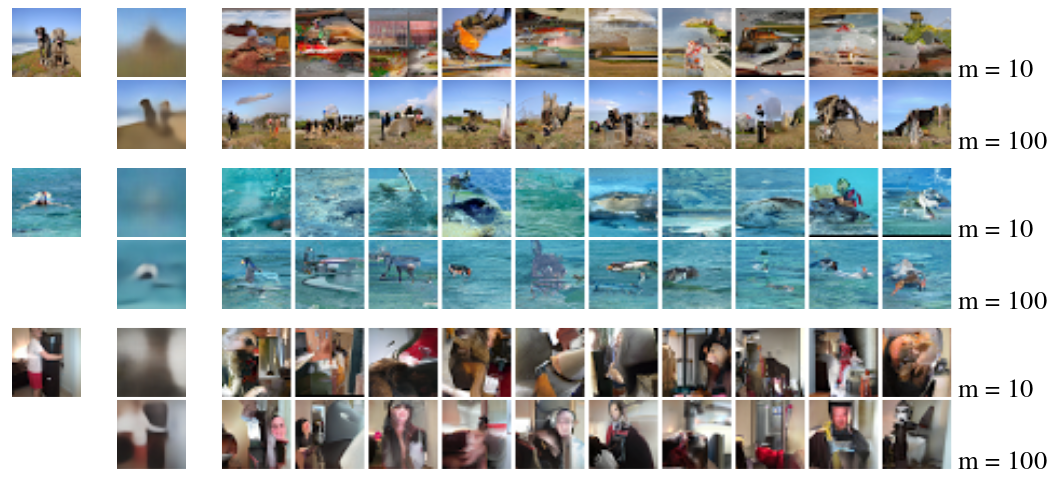
\includegraphics[width=0.8\textwidth]{fig/example_superres_2}
  \caption{Exemplo de aplicação do modelo probabilístico PixelNN. \citep{Oord16}}
  \label{fig:example2}
\end{center}
\end{figure}

O modelo de super-resolução é condicionado a um conjunto de
descrições $\boldsymbol{h}$, de modo que a distribuição condicional é dada
por:
\begin{equation}
\label{eqn:prodcnncond}
p(x|\boldsymbol{h}) = \prod_{i=1}^{n^2}p(x_i|x_1,...,x_{i-1}|\boldsymbol{h}).
\end{equation}
Desta forma, as ativações das camadas convolucionais dependem de $\boldsymbol{h}$,
antes de passarem pela função de não-linearidade. Se $\boldsymbol{h}$ contiver
informações referentes a classes de características encontradas nas imagens, todas as camadas terão um \textit{bias} que determina
a dependência destas classes. Por outro lado, se $\boldsymbol{h}$ for mapeado
para uma representação espacial $\boldsymbol{s}=m(\boldsymbol{h})$, onde $m$ é uma rede
deconvolucional, as camadas convolucionais terão \textit{biases} dependentes da localização
das estruturas contidas em $\boldsymbol{h}$, presentes na imagem. Assim, a equação \ref{eqn:actvcnn}
ganha a seguinte forma \citep{Oord16}:
\begin{equation}
\label{eqn:actvcnncond}
y = tanh(W_{k,f} * x + V_{k,f}*\boldsymbol{s})\bigodot \sigma(W_{k,g}*x + V_{k,g}*\boldsymbol{s}).
\end{equation}

O modelo de rede condicional proposto por \cite{DahlNS17} representa o estado da arte em modelos convolucionais para
super-resolução de múltiplas imagens. O modelo é composto de uma rede condicionante, do tipo ResNet \citep{He2016}
e uma rede \textit{prior}, do tipo \textit{Gated PixelNN} \citep{Oord16}.
A rede condicionante realiza o mapeamento de uma imagem de baixa resolução para uma estrutura probabilística
de alta resolução. Assim, ela permite compor a estrutura da imagem de alta resolução através da distribuição
de probabilidade marginal dos \textit{pixels} na imagem de baixa resolução. A rede \textit{prior} adiciona detalhes de alta resolução
para tornar as saídas mais realísticas. 

Para treinar um modelo que mapeie uma imagem $x$ de baixa resolução em uma imagem $y$ de alta resolução,
dada uma imagem $y^*$ considerada a realidade desejada, é preciso otimizar os parâmetros
$\theta$ da distribuição condicional $p_{\theta}(\boldsymbol{y}|\boldsymbol{x})$ de modo
a maximizar a função objetivo condicional dada por \citep{DahlNS17}:
\begin{equation}
\label{eqn:objfunc}
O(\theta|\mathcal{D})= \sum_{(\boldsymbol{x},\boldsymbol{y^*})\in \mathcal{D}} log p(\boldsymbol{y^*}|\boldsymbol{y}),
\end{equation}
onde $\mathcal{D} \equiv \{(\boldsymbol{x}^{(i)},\boldsymbol{y}^{*(i)})\}_{i=1}^N$ denota o conjunto
de treinamento da rede, composto pelos pares de imagens de baixa resolução e de alta resolução que representa
a realidade observada.

Dada uma imagem $ \boldsymbol{x} \in \mathbb{R}^L $, $A_i(\boldsymbol{x}) : \mathbb{R}^L \rightarrow \mathbb{R}^K$
representa a rede condicionante capaz de prever um vetor de valores que correspondem a $K$ valores
possíveis que o $i$-ésimo \textit{pixel} de saída pode assumir. Analogamente,
$B_i(\boldsymbol{y}_{<i}) : \mathbb{R}^{i-1} \rightarrow \mathbb{R}^K$ representa a rede \textit{prior}
capaz de prever um vetor de valores do $i$-ésimo \textit{pixel}. A previsão da distribuição
sobre o $i$-ésimo \textit{pixel} de saída é obtida pela adição dos dois conjuntos de saída e aplicação
do operador de \textit{softmax}:

\begin{equation}
\label{eqn:cnnpred}
p(y_i|\boldsymbol{x},\boldsymbol{y}_{<i}) = softmax(A_i(\boldsymbol{x}) + B_i(\boldsymbol{y}_{<i})).
\end{equation}
O operador \textit{softmax} é uma generalização da regressão logística. Na regressão logística se assume que a classificação 
admite um entre dois valores: $y^{(i)} \in \{ 0,1\}$. A regressão \textit{softmax} permite lidar com
$y^{(i)} \in \{ 0,...,K\}$, onde $K$  é o número de classes \citep{Nielson15}.

O algoritmo Gradiente Descente Estocástico é usado para otimizar os parâmetros $A$ e $B$, a fim de maximizar
a \textit{log-likelihood} da Equação \ref{eqn:objfunc}. O aprendizado da rede ocorre pela otimização da função de custo entre
as predições do modelo (Equação \ref{eqn:cnnpred}) e os valores discretos da imagem que representa
a realidade $y_i^* \in \{1...K\}$:

\begin{equation}
\label{eqn:cnncostfunc}
O = \sum_{(\boldsymbol{x},\boldsymbol{y^*})\in \mathcal{D}} \sum_{i=1}^{M}\big(\zeta [\boldsymbol{y_i^*}]^T(A_i(\boldsymbol{x}) + B_i(\boldsymbol{y}_{<i}^*))
-lse(A_i(\boldsymbol{x}) + B_i(\boldsymbol{y}_{<i}^*))) \big).
\end{equation}

Os experimentos realizados por \cite{DahlNS17} compreenderam o treinamento do modelo condicionado
com o conjunto de dados \textit{CelebA} \citep{liu15}, o qual é composto por $200K$ imagens de
faces de pessoas consideradas celebridades. Os autores redimensionaram as imagens de
$32$ x $32$ para $8$ x $8$ para obter a mesma imagem, porém borrada. Com isto, os
pares de treinamento da rede foram formados. A Figura \ref{fig:example1} apresenta um exemplo
de resultado obtido pelo modelo proposto. A coluna da esquerda mostra as imagens de baixa
resolução, em tamanho $8$x$8$, usadas como entrada para o modelo, a coluna central mostra o
resultado obtido com o modelo, em tamanho $32$ x $32$, e a coluna da direita apresenta o imagem
real.
\begin{figure}[ht!]
\begin{center}
  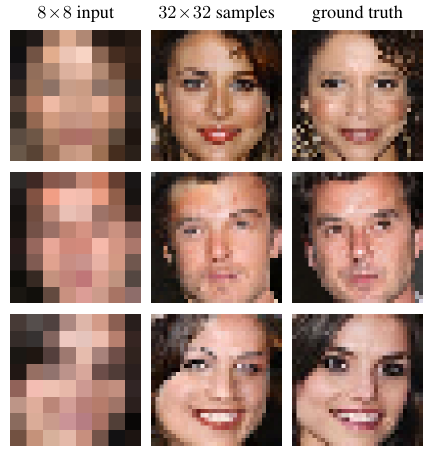
\includegraphics[width=0.4\textwidth]{fig/example_superres_1}
  \caption{Ilustração do modelo probabilístico. \citep{DahlNS17}}
  \label{fig:example1}
\end{center}
\end{figure}

Mais recentemente, os avanços das pesquisas do Google em \textit{Deep Learning} disponibilizaram
ferramentas de implementação de diferentes algoritmos de aprendizagem de máquina. Dentre estas
ferramentas está o \textit{Framework} de \textit{Deep Learning} TensorFlow, no qual os modelos
de redes convolucionais podem ser implementados e testados.

\section{Resumo}

Neste capítulo foram revisados os estados da arte em inversão sísmica acústica e modelos
de rede convolucional para super-resolução.
O próximo capítulo irá definir a proposta de pesquisa, apresentar o plano de trabalho e concluir com as perspectivas de
contribuição.
